%%%%%%%%%%%%%%%%%%%%%%%%%%%%%%%%%%%%%%%%%%%%%%%%%%%%%%%%%%%%%%%%
%%                                                            %%
%%   essentialsOfLatin, Italian translation 2017              %%
%%                                                            %%
%% From:  Henry C. Pearson, Essentials Of Latin For Beginners %%
%%        (1915, New York, American Book Company)             %%
%%                                                            %%
%%    https://archive.org/details/essentialslatin04peargoog   %%
%%                                                            %%
%% Translated by g.p.ciceri <gp.ciceri@gmail.com>             %%
%% ---------------------------------------------------------- %%
%% This translation is Licensed under                         %%
%% Creative Commons Attribution-ShareAlike 4.0 International  %%
%% https://creativecommons.org/licenses/by-sa/4.0/            %%
%%                                                            %%
%%%%%%%%%%%%%%%%%%%%%%%%%%%%%%%%%%%%%%%%%%%%%%%%%%%%%%%%%%%%%%%%

% āēīōū
% ăĕĭŏŭ




\documentclass[nols]{tufte-handout}

%\geometry{showframe} % display margins for debugging page layout

\usepackage{fontspec}
\usepackage{ifxetex}
\setmainfont[Path=./fonts/palatino-linotype/, ItalicFont=palai.ttf, BoldFont=palab.ttf]{pala.ttf}


% \defaultfontfeatures{Mapping=tex-text}
% \setromanfont[Path=./fonts/TeX-Gyre-Schola/,Mapping=tex-text]{TeX Gyre Schola}
% \setsansfont[Path=./fonts/TeX-Gyre-Heros/,Scale=MatchLowercase,Mapping=tex-text]{TeX Gyre Heros}
% \setmonofont[Path=./fonts/TeX-Gyre-Cursor/,Scale=MatchLowercase]{TeX Gyre Cursor}

\usepackage{lipsum}
\usepackage{url}
\usepackage{longtable}
\usepackage{stackengine}

\usepackage{graphicx} % allow embedded images
  \setkeys{Gin}{width=\linewidth,totalheight=\textheight,keepaspectratio}
  \graphicspath{{graphics/}} % set of paths to search for images
\usepackage{amsmath}  % extended mathematics
\usepackage{booktabs} % book-quality tables
\usepackage{units}    % non-stacked fractions and better unit spacing
\usepackage{multicol} % multiple column layout facilities
\usepackage{lipsum}   % filler text
\usepackage{fancyvrb} % extended verbatim environments
  \fvset{fontsize=\normalsize}% default font size for fancy-verbatim environments

% Standardize command font styles and environments
\newcommand{\doccmd}[1]{\texttt{\textbackslash#1}}% command name -- adds backslash automatically
\newcommand{\docopt}[1]{\ensuremath{\langle}\textrm{\textit{#1}}\ensuremath{\rangle}}% optional command argument
\newcommand{\docarg}[1]{\textrm{\textit{#1}}}% (required) command argument
\newcommand{\docenv}[1]{\textsf{#1}}% environment name
\newcommand{\docpkg}[1]{\texttt{#1}}% package name
\newcommand{\doccls}[1]{\texttt{#1}}% document class name
\newcommand{\docclsopt}[1]{\texttt{#1}}% document class option name
\newenvironment{docspec}{\begin{quote}\noindent}{\end{quote}}% command specification environment

% concetti morfosintattici
\usepackage{xspace} 
\newcommand{\noun}{\textsc{sostantivo}\xspace}
\newcommand{\nouns}{\textsc{sostantivi}\xspace}
\newcommand{\adject}{\textsc{aggettivo}\xspace}
\newcommand{\adjects}{\textsc{aggettivi}\xspace}
\newcommand{\gnumber}{\textsc{numero}\xspace}
\newcommand{\gnumbers}{\textsc{numeri}\xspace}
\newcommand{\gender}{\textsc{genere}\xspace}
\newcommand{\genders}{\textsc{generi}\xspace}
\newcommand{\gcase}{\textsc{caso}\xspace}
\newcommand{\gcases}{\textsc{casi}\xspace}
\newcommand{\tense}{\textsc{tempo}\xspace}
\newcommand{\mood}{\textsc{modo}\xspace}
\newcommand{\gverb}{\textsc{verbo}\xspace}
\newcommand{\gverbs}{\textsc{verbi}\xspace}
\newcommand{\adjective}{\textsc{aggettivo}\xspace}
\newcommand{\nom}{\textsc{nom}\xspace}
\newcommand{\gen}{\textsc{gen}\xspace}
\newcommand{\dat}{\textsc{dat}\xspace}
\newcommand{\acc}{\textsc{acc}\xspace}
\newcommand{\voc}{\textsc{voc}\xspace}
\newcommand{\abl}{\textsc{abl}\xspace}
\newcommand{\gexit}{\textsc{uscita}\xspace}
\newcommand{\gexits}{\textsc{uscite}\xspace}
\newcommand{\declinazione}{\textsc{declinazione}\xspace}
\newcommand{\masc}{\textsc{maschile}\xspace}
\newcommand{\femm}{\textsc{femminile}\xspace}
\newcommand{\neut}{\textsc{neutro}\xspace}

\newcommand{\indic}{\textsc{indicativo}\xspace}
\newcommand{\imper}{\textsc{imperativo}\xspace}
\newcommand{\gcong}{\textsc{congiuntivo}\xspace}
\newcommand{\ott}{\textsc{ottativo}\xspace}
\newcommand{\partic}{\textsc{participio}\xspace}
\newcommand{\infin}{\textsc{infinito}\xspace}

\newcommand{\pres}{\textsc{presente}\xspace}
\newcommand{\imperf}{\textsc{imperfetto}\xspace}
\newcommand{\aor}{\textsc{aoristo}\xspace}
\newcommand{\fut}{\textsc{futuro}\xspace}
\newcommand{\perf}{\textsc{perfetto}\xspace}
\newcommand{\pperf}{\textsc{piuccheperfetto}\xspace}

\newcommand{\sing}{\textsc{singolare}\xspace}
\newcommand{\plur}{\textsc{plurale}\xspace}
\newcommand{\dual}{\textsc{duale}\xspace}

\newcommand{\si}{\textsc{sing}\xspace}
\newcommand{\pl}{\textsc{plur}\xspace}
\newcommand{\du}{\textsc{dual}\xspace}

\newcommand{\att}{\textsc{attivo}\xspace}
\newcommand{\med}{\textsc{medio}\xspace}
\newcommand{\pass}{\textsc{passivo}\xspace}
\newcommand{\medpass}{\textsc{medio-passivo}\xspace}


% italianitudini
\renewcommand{\figurename}{Figura}
\renewcommand{\tablename}{Tabella}
\renewcommand{\contentsname}{Indice}

% fix per un qualche problema
\ifxetex
  \newcommand{\textls}[2][5]{%
    \begingroup\addfontfeatures{LetterSpace=#1}#2\endgroup
  }
  \renewcommand{\allcapsspacing}[1]{\textls[15]{#1}}
  \renewcommand{\smallcapsspacing}[1]{\textls[10]{#1}}
  \renewcommand{\allcaps}[1]{\textls[15]{\MakeTextUppercase{#1}}}
  \renewcommand{\smallcaps}[1]{\smallcapsspacing{\scshape\MakeTextLowercase{#1}}}
  \renewcommand{\textsc}[1]{\smallcapsspacing{\textsmallcaps{#1}}}
\fi

% too many float...
\extrafloats{100}

\title{Essentials Of Latin. Elementi di Latino. \newline Lezione XXI - Imperfetto e Futuro Indicativo Passivo per la I e II coniugazione. Ablativo di Modo.}

\author[gpciceri]{a cura di Milagathòs: Milo's help to enjoy humanities.}

\date{21 Gennajo 2017} % without \date command, current date is supplied


\begin{document}

\hyphenation{co-niu-ga-zio-ne}

\maketitle% this prints the handout title, author, and date

\begin{marginfigure}[-2.5cm]
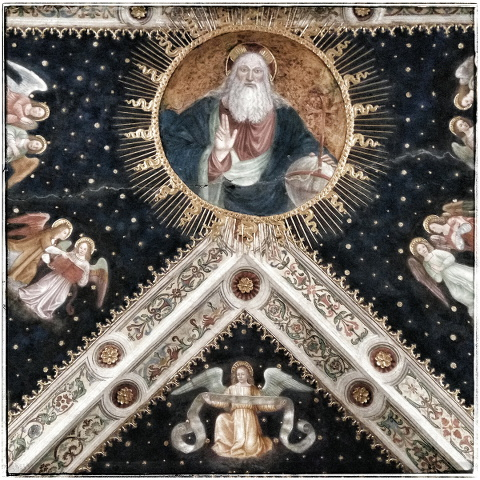
\includegraphics{smallthumb-lesson_XI.jpeg}
\setfloatalignment{b}
\end{marginfigure}


\begin{abstract}
\noindent
Queste lezioni riprendono il testo introduttivo al Latino di Pearson\cite{pearson1915}, del quale seguono la numerazione; la struttura di ogni lezione è piuttosto regolare: inizia con \textsc{cenni di morfologia e di sintassi latina}, seguita da un \textsc{piccolo vocabolario} per il lessico; ci sono infine vari \textsc{esercizi} di traduzione e di composizione latina.

\bigskip
\noindent
Lezione XXI - Imperfetto e Futuro Indicativo Passivo per la I e II coniugazione. Ablativo di Modo.
\end{abstract}

%\printclassoptions


\newthought{146. Prima e Seconda Coniugazione, indicativo imperfetto passivo.} 

\begin{fullwidth}
\begin{table}[!htbp]
  \centering
  \begin{tabular}{l l l l l}
    %\toprule
	\multicolumn{5}{c}{\textsc{I e II Coniugazione - Indicativo Imperfetto Passivo}} \\
	\multicolumn{2}{c}{\textsc{Singolare}} & \hspace{10mm} & \multicolumn{2}{c}{\textsc{Singolare}} \\

    \textsc{1.} & amā\textbf{bar},                     \textit{io ero amato}    & \hspace{10mm} & \textsc{1.} & monē\textbf{bar}, \textit{io ero ammonito} \\
    \textsc{2.} & amā\textbf{bāris}, amā\textbf{bāre}, \textit{tu eri amato}    & \hspace{10mm} & \textsc{2.} & monē\textbf{bāris}, monē\textbf{bāre}, \textit{tu eri ammonito} \\
    \textsc{3.} & amā\textbf{bātur},                   \textit{egli era amato}  & \hspace{10mm} &  \textsc{3.} & monē\textbf{bātur}, \textit{egli era ammonito}\\
	
	\multicolumn{2}{c}{\textsc{Plurale}} & \hspace{10mm} & \multicolumn{2}{c}{\textsc{Plurale}} \\

	\textsc{1.} & amā\textbf{bāmur},                     \textit{noi eravamo amati}    & \hspace{10mm} & \textsc{1.} & monē\textbf{bāmur}, \textit{noi eravamo ammoniti} \\
    \textsc{2.} & amā\textbf{bāminī}, amā\textbf{bāre}, \textit{voi eravati amati}    & \hspace{10mm} & \textsc{2.} & monē\textbf{bāminī}, monē\textbf{bāre}, \textit{voi eravate ammoniti} \\
    \textsc{3.} & amā\textbf{bantur},                   \textit{essi erano amati}  & \hspace{10mm} &  \textsc{3.} & monē\textbf{bantur}, \textit{essi erano ammoniti}\\
	
	\multicolumn{5}{c}{\textemdash} \\
	
	\multicolumn{5}{c}{\textsc{I e II Coniugazione - Indicativo Futuro Passivo}} \\
	\multicolumn{2}{c}{\textsc{Singolare}} & \hspace{10mm} & \multicolumn{2}{c}{\textsc{Singolare}} \\

    \textsc{1.} & amā\textbf{bor},                     \textit{io sarò amato}    & \hspace{10mm} & \textsc{1.} & monē\textbf{bor}, \textit{io sarò ammonito} \\
    \textsc{2.} & amā\textbf{beris}, amā\textbf{bāere}, \textit{tu sarai amato}    & \hspace{10mm} & \textsc{2.} & monē\textbf{beris}, monē\textbf{bere}, \textit{tu sarai ammonito} \\
    \textsc{3.} & amā\textbf{bitur},                   \textit{egli sarà amato}  & \hspace{10mm} &  \textsc{3.} & monē\textbf{bitur}, \textit{egli sarà ammonito}\\
	
	\multicolumn{2}{c}{\textsc{Plurale}} & \hspace{10mm} & \multicolumn{2}{c}{\textsc{Plurale}} \\

	\textsc{1.} & amā\textbf{bimur},                     \textit{noi saremo amati}    & \hspace{10mm} & \textsc{1.} & monē\textbf{bāmur}, \textit{noi saremo ammoniti} \\
    \textsc{2.} & amā\textbf{biminī}, amā\textbf{bāre}, \textit{voi sarete amati}    & \hspace{10mm} & \textsc{2.} & monē\textbf{biminī}, monē\textbf{bāre}, \textit{voi sarete ammoniti} \\
    \textsc{3.} & amā\textbf{buntur},                   \textit{essi saranno amati}  & \hspace{10mm} &  \textsc{3.} & monē\textbf{buntur}, \textit{essi saranno ammoniti}\\
	
    %\bottomrule
  \end{tabular}
  %\caption{}
  \label{tab:normaltab}
  %\zsavepos{pos:normaltab}
\end{table}
\end{fullwidth}


\newthought{Osservazioni}
\begin{itemize}
\item[\textsc{1.}] Le uscite personali sono le stesse del presente passivo (139.).  
\item[\textsc{2.}] La vocale prima delle uscite personali è \textbf{a} nell'imperfetto, nel futuro invece cambia. Qual è la vocale caratteristica del futuro?  
\item[\textsc{3.}] L'imperfetto e il futuro passivo sono formati a partire dal tema del presente \textbf{amā-} e \textbf{monē-}, aggiungendo rispettivamente \textbf{-bar} e \textbf{-ber}.  
\end{itemize}

% āēīōū
% ăĕĭŏŭ

\newthought{147. Frasi Modello.} Esamina le seguenti frasi:
\begin{itemize}
\item[\textsc{1.}] \textbf{Agricola cum cura arat}, \textit{l'agricoltore ara con cura (accuratamente)}.  
\item[\textsc{2.}] \textbf{Agricola magna cum cura arat}, \textit{l'agricoltore ara con grande cura (molto accuratamente)}.  
\item[\textsc{3.}] \textbf{Agricola magna cura arat}, \textit{l'agricoltore ara con grande cura (molto accuratamente)}.    
\end{itemize}


\newthought{Osservazioni} 
\begin{itemize}
\item[\textsc{1.}] Le espressioni in latino \textbf{cum cura, magna cum\sidenote{la preposizione \textit{monosillabica} viene scritta tra l'aggettivo e il nome} cura, magna cura}, indicano il \textit{modo} dell'azione espressa dal verbo (cioè il \textit{come} l'azione del verbo è compiuta).  
\item[\textsc{2.}] Le espressioni \textbf{magna cum cura} e \textbf{magna cura} vengono tradotti allo stesso modo.      
\item[\textsc{2.}] Queste espressioni possono venir tradotte anche da un avverbio.      
\end{itemize}


\newthought{148. Regola \textemdash Ablativo di Modo.} Il Complemento di Modo è espresso con l'\abl preceduto dalla preposizione \textbf{cum}, ma se un aggettivo viene usato con il nome che funge da complemento, il \textbf{cum} può venire tralasciato.

\newthought{149. Vocabolario}

\begin{multicols}{2}
    \noindent \hangindent=1em \textbf{studium, -i}, n., \textit{zelo, impazienza}.  \\
    \noindent \hangindent=1em \textbf{cura, -ae}, f., \textit{preoccupazione}.  \\
	\noindent \hangindent=1em \textbf{obses, obsidis}, m. e f., \textit{ostaggio, prigioniero}.  \\
	\noindent \hangindent=1em \textbf{multitudo, multitudinis}, f., \textit{moltitudine, folla}.  \\
	\noindent \hangindent=1em \textbf{imperium, -i}, n., \textit{comando, potere (militare)}.  \\
	\noindent \hangindent=1em \textbf{imperator, -oris}, m., \textit{comandante (militare) in capo}.  \\
	\noindent \hangindent=1em \textbf{conloco, -as, avi, -atum, -are}, \textit{mettere, collocare, disporre}.  \\
	\noindent \hangindent=1em \textbf{compleo, -es, -evi, -etum, -ēre}, \textit{riempire, completare}.  \\
    \noindent \hangindent=1em \textbf{diu}, avv. \textit{a lungo, per un lungo tempo}.     \\
	
\end{multicols}


\newthought{150. Esercizi di Ripasso}
\\
\textsc{I.} \quad
\textsc{1.}~Equitum celeritate Romani terrentur. \quad
\textsc{2.}~Caesar legato equum pulchrum dat. \quad
\textsc{3.}~Legato a Cesare equus pulcher datur. \quad
\textsc{4.}~Hieme frumenti inopia hostes laborabant. \quad
\textsc{5.}~Magna urbs pars a Gallis occupatur. \quad
\textsc{6.}~Milites a rege in hiberna convocantur. \quad
\\
\textsc{II.} \quad
\textsc{1.}~Soffrimmo per molte ferite. \quad
\textsc{2.}~Nella notte il console prese possesso della montagna. \quad
\textsc{3.}~I ragazzi pigri non sono lodati da mio padre. \quad
\textsc{4.}~I Galli sono spaventati dalla velocità e dal coraggio dei soldati di Roma.

\newthought{145. Esercizi}
\\
\textsc{I.} \quad
\textsc{1.}~Laudabat, laudabatur; videbunt, videbuntur. \quad
\textsc{2.}~Portabamus, portabamur; superabis, superaberis. \quad
\textsc{3.}~In agris laborabunt magno cum studio. \quad
\textsc{4.}~In castris cum cura legio conlocabitur. \quad
\textsc{5.}~In colle diu cum hostibus dimicabant. \quad
\textsc{6.}~Legio a duce propter virtutem laudatur. \quad
\textsc{7.}~Caesari imperium dabitur. \quad
\textsc{8.}~Urbem equitum multitudine complevit. \quad
\textsc{9.}~Liberos multos obsides Caesari Galli dederant. \quad
\textsc{10.}~Equitesne a duce laudabuntur? 
\\
\textsc{II.} \quad
\textsc{1.}~Tu vedrai, tu sarai visto. \quad
\textsc{2.}~State lodando? Sarà maledetto. \quad
\textsc{3.}~Furono feriti dalla fanteria con le spade. \quad
\textsc{4.}~All'alba i Romani combatterono ardentemente. \quad
\textsc{5.}~Una gran parte delle armi era stata portata con molta cura nell'accampamento. \quad
\textsc{6.}~Molti soldati erano stati visti vicino al ponte.

\newthought{(447.) Lettura. Un Padre Severo} 
\\
Brutus et Valerius consules Romani erant et cum Tarquinio rege pugnabant. Sed mali filii Bruti
contra patrem a Tarquinio incitabantur. Cum paucis coniuratis Romae imperium Tarquinio domino dare parabant.
Sed per Bruti servum fidum, quod periculo terrebatur, consuli nomina coniuratorum nuntiantur.
A consule filii cum coniuratis in collem Capitolinum magna cum celeritate convocantur.
Tum Brutus homines superbos culpat quod contra urbem armantur. Pater miser filiorum vitam non servavit.
Tum milites homines malos gladiis necaverunt. Sed Bruti, patris fortissimi, magna virtus a Romanis gratis semper laudabitur.

\begin{figure}[!b]
  %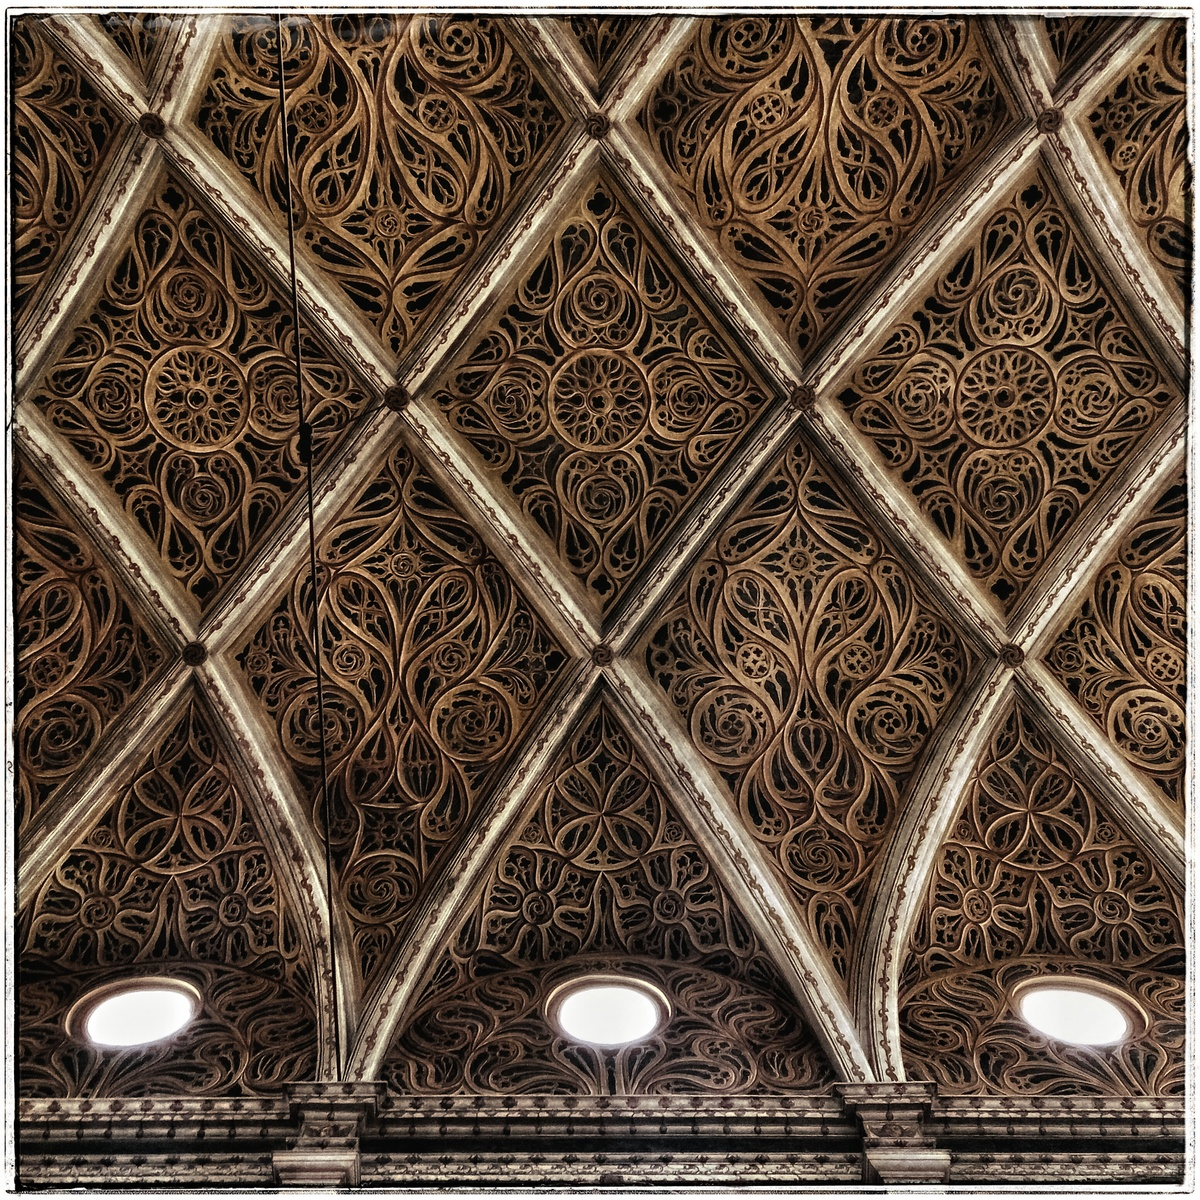
\includegraphics{thumb-lesson_XXI.jpeg}
  %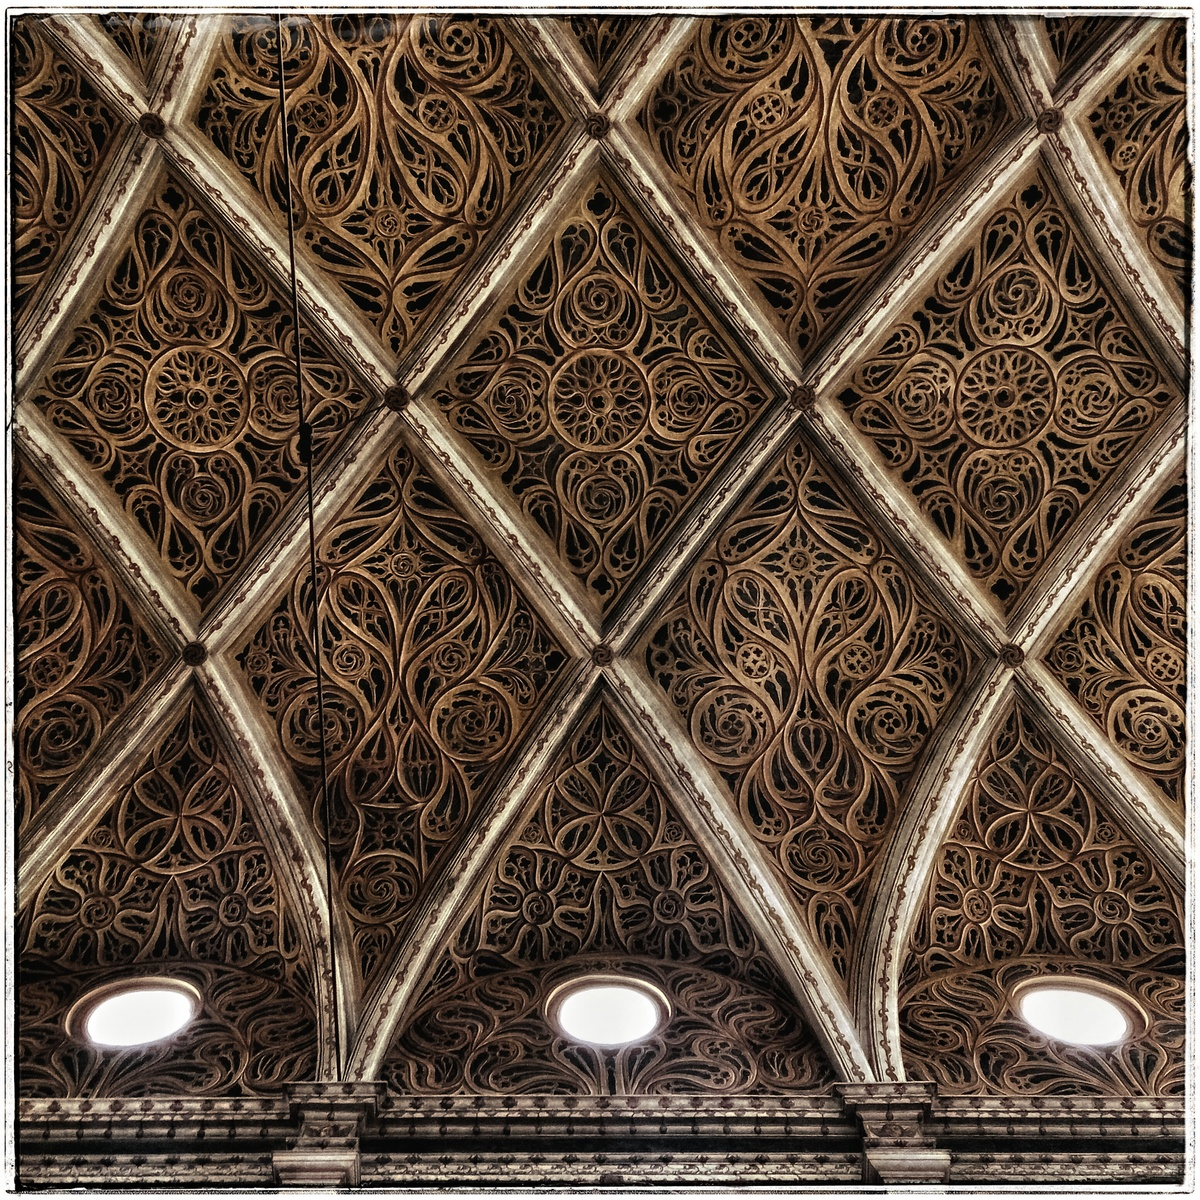
\includegraphics[width=0.9\linewidth]{thumb-lesson_XXI.jpeg}
  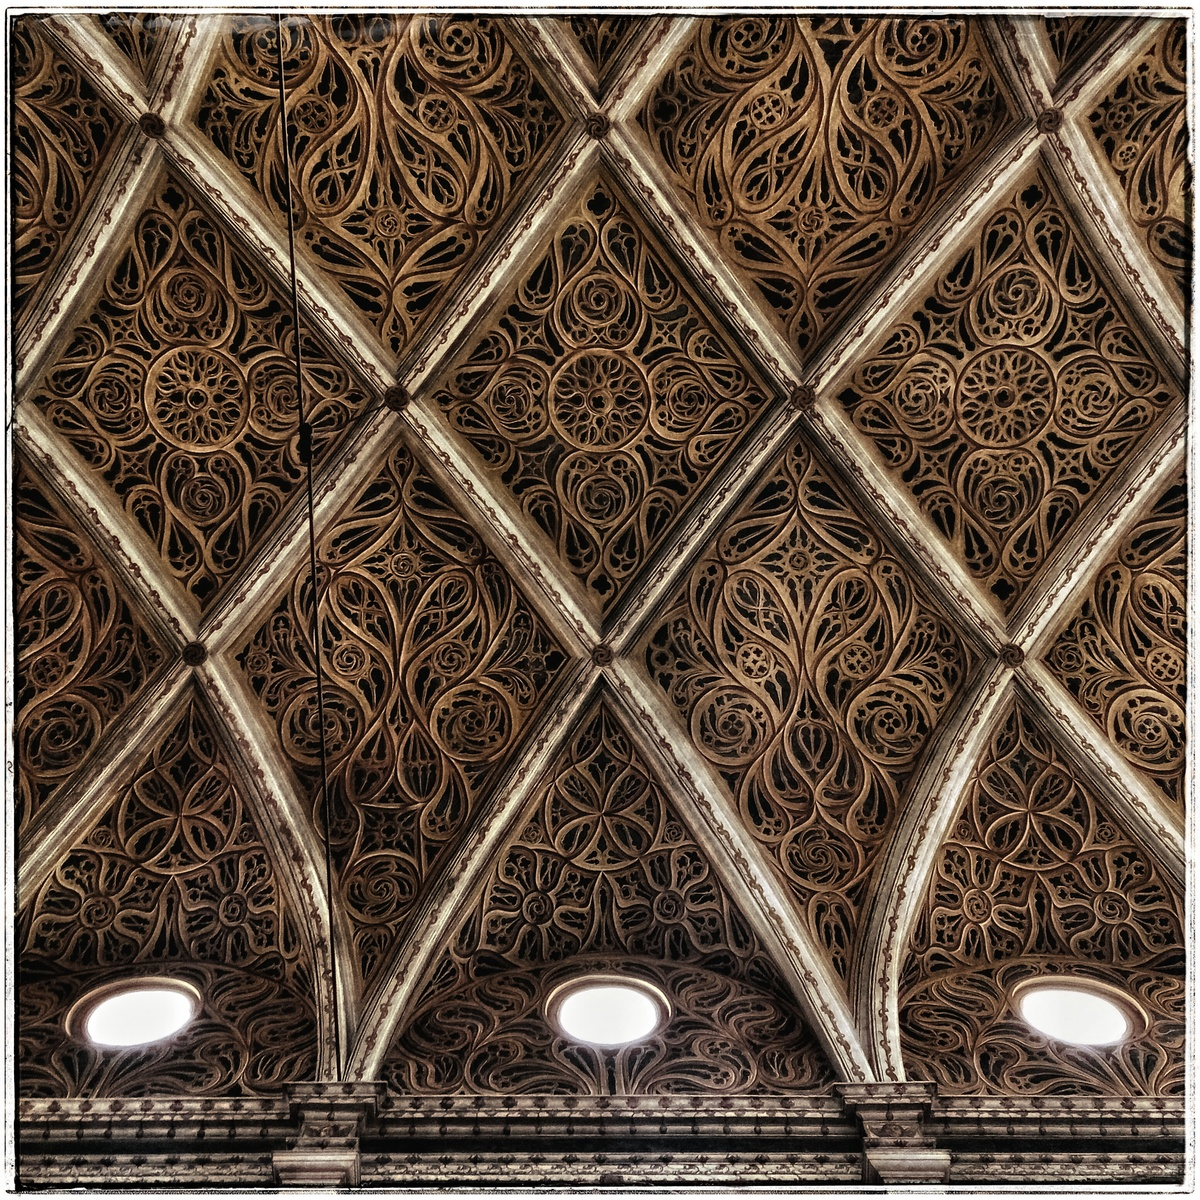
\includegraphics{thumb-lesson_XXI.jpeg}
  \caption{Milano: San Maurizio al Monastero Maggiore}
  \label{fig:textfig}
  %\zsavepos{pos:textfig}
  %\setfloatalignment{b}
\end{figure}

 

\nobibliography{latinBiblio}
\bibliographystyle{alpha}


\end{document}
